\section[Some Special Functions]{\hyperlink{toc}{Some Special Functions}}

\subsection{Power Series, Revisited}
Recall our definition of power series (Definition \ref{def:3.38}), functions of the form:
\begin{align*}
    f(x) = \sum_{n=0}^\infty c_n x^n.
\end{align*}
Also recall the radius of convergence (Theorem \ref{thm:3.39}) of such power series, defined as:
\begin{align*}
    R = \frac{1}{\limsup_{n \rightarrow \infty}\sqrt[n]{\abs{c_n}}}.
\end{align*}
Note that if $\limsup_{n \rightarrow \infty}\sqrt[n]{\abs{c_n}} = \infty$, then $R = 0$, and if $\limsup_{n \rightarrow \infty}\sqrt[n]{\abs{c_n}} = 0$, then $R = \infty$. The series converges absolutely for $\abs{x} < R$ and diverges for $\abs{x} > R$.

\begin{figure}[htbp]
    \centering
    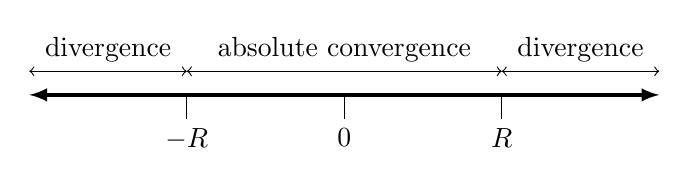
\begin{tikzpicture}[scale=2]
        \draw[latex-latex, very thick] (-2, 0) -- (2, 0);
        \draw[] (0, 0) -- (0, -0.15);
        \draw[] (1, 0) -- (1, -0.15);
        \draw[] (-1, 0) -- (-1, -0.15);
        \node[below] at (0, -0.15) {$0$};
        \node[below] at (1, -0.15) {$R$};
        \node[below] at (-1, -0.15) {$-R$};
        \draw[<->] (1, 0.15) -- (-1, 0.15);
        \draw[<->] (1, 0.15) -- (2, 0.15);
        \draw[<->] (-1, 0.15) -- (-2, 0.15);
        \node[above] at (0, 0.15) {absolute convergence};
        \node[above] at (1.5, 0.15) {divergence};
        \node[above] at (-1.5, 0.15) {divergence};
    \end{tikzpicture}
    
    \caption{Visualization of the radius of convergence for $f(x) = \sum_{n=0}^\infty c_nx^n$, $x \in \RR$.}
    \label{fig49}
\end{figure}

\begin{theorem}{}{8.1}
    If $\sum_{n=0}^\infty c_nx^n$ converges for $\abs{x} < R$, let $f(x) = \sum_{n=0}^\infty c_n x^n$ for $\abs{x} < R$. Then, the series converges uniformly on $[-R + \e, R - \e]$ for any $\e > 0$, $f$ is differentiable (and hence continuous) on $(-R, R)$ and $f'(x) = \sum_{n=0}^\infty nc_nx^{n-1}$. 
\end{theorem}

\begin{nproof}
    We first show the uniform convergence on $[-R + \e, R - \e]$. For $\abs{x} \leq R - \e$, we have that $\abs{c_nx^n} \leq \abs{x_n}(R - \e)^n$. Since $\sum_n \abs{c_n}(R - \e)^n < \infty$ (by the assumed absolute convergence on $(-R, R)$), we have that $\sum_n c_nx^n$ converges uniformly in $\abs{x} \leq R - \e$ by the M-test (Theorem \ref{thm:7.10}).

    We next prove the claim about the differentiability/derivative of $f$. The radius of convergence of $\sum_n nc_n x^{n-1}$ is:
    \begin{align*}
        \frac{1}{\limsup_{n \rightarrow \infty}\sqrt[n]{\abs{nc_n}}} = \frac{1}{\limsup_{n \rightarrow \infty}\sqrt[n]{\abs{c_n}}} = R
    \end{align*}
    so since $f$ converges in $(-R, R)$, so does $\sum_n nc_nx^{n-1}$. Now, let $s_n(x) = \sum_{m=0}^n c_mx^m$. Then, by the linearity of the derivative we have that $s_n'(x) = \sum_{m=1}^n mc_mx^{m-1}$. By the first part of the proof, we have that $s_n'(x) \rightarrow \sum_{m=1}^\infty mc_mx^{m-1}$ uniformly on $[-R + \e, R - \e]$. Since $s_n(x) \rightarrow f(x)$ uniformly, by Theorem \ref{thm:7.17}, we have that $f'$ exists on $[-R +\e, R - \e]$ and $f'(x) = \sum_{m=1}^\infty mc_mx^{m-1}$. Since $\e$ is arbitrary, $f'$ exists and is equal to $\sum_{m=1}^\infty mc_mx^{m-1}$ for all $x \in (-R, R)$. \qed 
\end{nproof}
\noindent As a remark, note that we can (interestingly) prove the differentiability of $f$ on $(-R, R)$ from the uniform convergence on $[-R + \e, R - \e]$.

\begin{ncorollary}{}{}
    If $f(x) = \sum_{n=0}^\infty c_nx^n$ converges for $\abs{x} < R$, then $f^{(k)}(x)$ exists for all $k \in \NN$ and for all $x \in (-R, R)$. It is given by:
    \begin{align*}
        f^{(k)}(x) = \sum_{n=k}^\infty n(n-1)\ldots(n-k+1)c_nx^{n-k} \quad (*)
    \end{align*}
    and consequently, we have that $c_k = \frac{f^{(k)(0)}}{k!}$, so $f(x) = \sum_{n=0}^\infty \frac{f^{(n)}(0)}{n!}x^n$.
\end{ncorollary}
\noindent Compare the above Corollary to Taylor's theorem (Theorem \ref{thm:5.15}). Here, we take our taylor polynomial and extend it to an infinite series (the limit of polynomials). 

\begin{nproof}
    By Theorem \ref{thm:8.1}, we have that $f'(x) = \sum_{n=1}^\infty nc_nx^{n-1}$ and $f''(x) = \sum_{n=2}^\infty n(n-1)c_nx^{n-2}$ and so on. Setting $x = 0$ in $(*)$, we have that $f^{(k)}(0) = n(n-1)\ldots 1 c_n = n! c_k$, so $c_n = \frac{f^{(k)}(0)}{n!}$. \qed
\end{nproof}
\noindent Recall the definition of \emph{analytic functions}, which are infinite differentiable and can be represented as sums or series of derivatives evaluated at zero. 

\begin{nexample}{}{}
    As we discussed in Chapter 5, there are infinitely differentiable functions that are not analytic. Let:
    \begin{align*}
        f(x) = \begin{cases}
            \exp(-\frac{1}{x^2}) & x \neq 0
            \\ 0 & x = 0
        \end{cases}
    \end{align*}
    By Theorem \ref{thm:8.1}, $f$ is infinitely differentiable, and $f^{(n)}(0) = 0$ for all $n \in \NN$. But, $f(x) \neq 0$ except at $x = 0$. Hence, $f(x) \neq \sum_{n=0}^\infty \frac{f^{(n)}(0)}{n!}x^n$ except at $x = 0$. This is true despite the fact that the RHS converges to zero for all $x \in \RR$. 
\end{nexample}

\begin{nexample}{}{}
    Bump functions are continuous, infinitely differentiable functions of compact support (it is zero outside of a compact set). For example, 
    \begin{align*}
        f(x) = \begin{cases}
            \exp(-\frac{1}{1-x^2}) & x \in (-1, 1)
            \\ 0 & \abs{x} \geq 1
        \end{cases}
    \end{align*}
    is an example of a bump function. Such functions are very useful in the study of functional analysis and PDEs.
\end{nexample}
\begin{figure}[htbp]
    \centering
    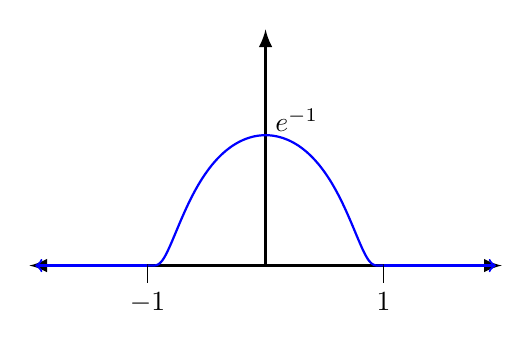
\begin{tikzpicture}[scale=1.5]
        \draw[-latex, very thick] (0, 0) -- (0, 2);
        \draw[latex-latex, very thick] (-2, 0) -- (2, 0);
        \draw[blue, thick, smooth, samples = 100, domain=-0.999:0.999, variable = \x] plot(\x, {3*exp(-1/(1-(\x)*(\x)))});
        \draw[->, blue, thick] (1, 0) -- (1.95, 0);
        \draw[->, blue, thick] (-1, 0) -- (-1.95, 0);
        \draw[] (1, 0) -- (1, -0.15);
        \draw[] (-1, 0) -- (-1, -0.15);
        \node[below] at (1, -0.15) {$1$};
        \node[below] at (-1, -0.15) {$-1$};
        \node[right] at (0, 1.23) {$e^{-1}$};
    \end{tikzpicture}
    
    \caption{Plot of the bump function $f$ from the above example.}
    \label{fig50}
\end{figure}

\noindent Before we continue, some remarks on the radius of convergence are in order. Of course, the definition of $R = \frac{1}{\limsup_{n \rightarrow \infty}\sqrt[n]{\abs{c_n}}}$ always holds. But in practice, the ratio test is much nicer to use (though it does not always work). We can make the observation that:
\begin{align*}
    \abs{\frac{c_{n+1}x^{n+1}}{c_nx^n}} = \abs{x}\abs{\frac{c_{n+1}}{c_n}} \rightarrow \abs{x}L
\end{align*}
Where we take the $n \rightarrow \infty$ limit in the final expression (assuming the limit exists). We have that the power series converges if $\abs{x} < \frac{1}{L}$ and diverges if $\abs{x} > \frac{1}{L}$. So, when the limit exists, we can write:
\begin{align*}
    R = \frac{1}{\linf\abs{\frac{c_{n+1}}{c_n}}}.
\end{align*}
In general, by Theorem 3.37 (not covered in lecture in 320, see Rudin), we have that:
\begin{align*}
    \frac{1}{\limsup_{n \rightarrow \infty}\abs{\frac{c_{n+1}}{c_n}}} \leq R \leq \frac{1}{\liminf_{n \rightarrow \infty}\abs{\frac{c_{n+1}}{c_n}}}
\end{align*}

\begin{theorem}{Abel's Theorem}{8.2}
    Suppose $\sum_{n=0}^\infty c_n$ converges (perhaps conditionally). Let $f(x) = \sum_{n=0}^\infty c_nx^n$. Then, $f(x)$ converges if $\abs{x} < 1$, and $\lim_{x \rightarrow 1^{-}}f(x) = \sum_{n=0}^\infty c_n$. 
\end{theorem}
\begin{nproof}
    For the first claim, we have that $\limsup_{n \rightarrow \infty}\sqrt[n]{\abs{c_n}} \leq 1$ so by the root test, $\sum_n c_n x^n$ has $R \geq 1$. The interesting case is when $R = 1$ (as if $R > 1$, then $f$ is continuous on $(-R, R)$ and the result follows immediately). In this case, $f(x)$ converges if $\abs{x} < 1$. Let $s_n = \sum_{m=0}^n c_m$ and $s = \sum_{m=0}^\infty c_m = \lim_{n \rightarrow \infty}s_n$. Let $s_{-1} = 0$. Then, we have that $s_n - s_{n-1} = c_n$ for $n \geq 0$.

    Let $\e > 0$. We wish to show that there exists $\delta > 0$ such that for $1 -\delta < x < 1$ we have that $\abs{f(x) - s} < \e$. We start with the partial sum of $f(x)$. For $\abs{x} < 1$, we have:
    \begin{align*}
        \sum_{m=0}^n c_mx^m &= \sum_{m=0}^n (s_m - s_{m-1})x^m
        \\ &= \sum_{m=0}^n s_mx^m - x\sum_{m=0}^{n-1}s_m x^m
        \\ &= (1-x)\sum_{m=0}^n s_mx^m + s_nx^{n+1}.
    \end{align*}
    Now, let $n \rightarrow \infty$. We then have that $s_nx^{n+1} \rightarrow 0$ as $s_n \rightarrow s$ and $x^{n+1} \rightarrow 0$. We then have that $f(x) = (1-x)\sum_{m=0}^n s_mx^m + 0$, and using that $\sum_{m=0}^\infty x^m = \frac{1}{1-x}$, we obtain that:
    \begin{align*}
        \abs{f(x) - s} = \abs{(1-x)\sum_{m=0}^\infty(s_m - s)x^m} \leq \abs{1 - x}\sum_{m=0}^\infty \abs{s_m - s}\abs{x}^m.
    \end{align*}
    Now, choose $N$ such that $m \geq N$ implies $\abs{s_m - s} < \frac{\e}{2}$. Let $x \in (0, 1)$, and then:
    \begin{align*}
        \abs{f(x) - s} \leq (1-x)\sum_{m=0}^N\abs{s_m - s}x^n + (1-x)\frac{\e}{2}\frac{1}{1-x}
    \end{align*}
    The second term on the RHS is bounded using the geometric series. The first term is a polyonimal in $x$ and hence continuous everywhere (including at $x = 1$). It equals $0$ at $x = 1$, so it has absolute value less than $\frac{\e}{2}$ if $x \in (1-\delta, 1)$ for some $\delta$. Hence:
    \begin{align*}
        \abs{f(x) - s} < \frac{\e}{2} + \frac{\e}{2} = \e
    \end{align*}
    \noindent See Rudin page 175 for an application of this Theorem to prove Theorem 3.51 in a different way. Not that for the case where $\sum_n c_n = \infty$, the theorem still holds, with $\lim_{x \rightarrow 1^-}\sum_{n=0}^\infty c_nx^n = \infty$. \qed
\end{nproof}

\begin{theorem}{}{8.3}
    Suppose $\sum_{i=1}^\infty \left(\sum_{j=1}^\infty \abs{a_{ij}}\right) < \infty$. Then, $\sum_{i=0}^\infty \sum_{j=0}^\infty a_{ij} = \sum_{j=0}^\infty \sum_{i=0}^\infty a_{ij}$ (and both converge).
\end{theorem}
\begin{nproof}
    Rudin uses an overly clever proof. See HW7Q2 for a more natural one. \qed
\end{nproof}

\begin{theorem}{}{8.4}
    Suppose $f(x) = \sum_{n=0}^\infty c_nx^n$ has radius of convergence $R$ (Taylor series of $f$ at 0/Maclaurin series). Let $\abs{a} < R$. Then, $f(x) = \sum_{n=0}^\infty \frac{f^{(n)}(0)}{n!}(x-a)^n$ for (at least) $\abs{x - a} < R - \abs{a}$. 
\end{theorem}
\begin{figure}[htbp]
    \centering
    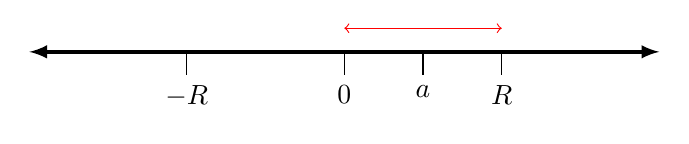
\begin{tikzpicture}[scale=2]
        \draw[latex-latex, very thick] (-2, 0) -- (2, 0);
        \draw[] (0, 0) -- (0, -0.15);
        \draw[] (1, 0) -- (1, -0.15);
        \draw[] (-1, 0) -- (-1, -0.15);
        \draw[] (0.5, 0) -- (0.5, -0.15);
        \node[below] at (0, -0.15) {$0$};
        \node[below] at (1, -0.15) {$R$};
        \node[below] at (-1, -0.15) {$-R$};
        \node[below] at (0.5, -0.15) {$a$};
        \draw[<->, red] (1, 0.15) -- (0, 0.15);
    \end{tikzpicture}
    
    \caption{Visualization of Theorem \ref{thm:8.4}. The new Taylor series around $x = a$ converges in the region up to the radius of convergence of the original series.}
    \label{fig51}
\end{figure}

\begin{nproof}
    We have that $f(x) = \sum_{n=0}^\infty c_n\left[(x - a) + a\right]^n = \sum_{n=0}^\infty c_n\sum_{m=0}^n \binom{n}{m}(x-a)^ma^{n-m}$, and we want to find a way to interchange the order of summation. By Theorem \ref{thm:8.3}, the interchange is permitted if:
    \begin{align*}
        \sum_{n=0}^\infty\sum_{m=0}^n \abs{c_n}\binom{n}{m}\abs{x-a}^m\abs{a}^{n-m} < \infty
    \end{align*}
    but the above is equaivalent to:
    \begin{align*}
        \sum_{n=0}^\infty \abs{c_n}\left(\abs{x - a} + \abs{a}\right)^n
    \end{align*}
    which converges if $\abs{x - a} + \abs{a} < R$. Therefore:
    \begin{align*}
        f(x) = \sum_{m=0}^\infty \sum_{n=m}^\infty c_n\binom{n}{m}a^{n-m}(x - a)^m
    \end{align*}
    over $n \geq m$. We need to show that these new coefficients $\left(\sum_{n=m}^\infty c_n\binom{n}{m}a^{n-m}\right)$ are equal to $\frac{f^{(m)}(a)}{m!}$. Expanding out, we have that:
    \begin{align*}
        \sum_{n=m}^\infty c_n\binom{n}{m}a^{n-m} = \frac{1}{m!}n(n-1)\ldots (n-m+1)c_na^{n-m} = \frac{1}{m!}f^{(m)}(a)
    \end{align*}
    where in the last equality we use Theorem \ref{thm:8.1}. We conclude that:
    \begin{align*}
        f(x) = \sum_{m=0}\frac{f^{(m)}(a)}{m!}(x-a)^m \text{ for } \abs{x - a} < R - \abs{a}
    \end{align*}
\end{nproof}

\begin{nexample}{}{}
    Let $f(x) = \sum_{n=0}^\infty x^n$. If $\abs{x} < 1$, then the series converges and $f(x) = \frac{1}{1-x}$ ($R = 1$). Choose $a = -\frac{1}{2}$ (we look at the Taylor serires around $x = -\frac{1}{2}$). For any $\abs{x} < 1$, we have that $f^{(n)}(x) = \frac{n!}{(1-x)^{n+1}}$, so therefore:
    \begin{align*}
        f^{(n)}(-\frac{1}{2}) = \frac{n!}{(1+\frac{1}{2})^{n+1}} = \left(\frac{2}{3}\right)^{n+1}n!.
    \end{align*}
    By Theorem \ref{thm:8.4}, we then have that:
    \begin{align*}
        f(x) = \sum_{n=0}^\infty \frac{\left(\frac{2}{3}\right)^{n+1}n!}{n!}(x - a)^n = \sum_{n=0}^\infty \left(\frac{2}{3}\right)^{n+1}(x + \frac{1}{2})^n
    \end{align*}
    which is valid for $\abs{x - (-\frac{1}{2})} < 1 - \abs{-\frac{1}{2}}$ and hence if $\abs{x + \frac{1}{2}} < \frac{1}{2}$. Note that in fact, $\sum_{n=0}^\infty\left(\frac{2}{3}\right)^{n+1}(x - a)^n$ converges whenever $\abs{\frac{2}{3}(x + \frac{1}{2})} < 1$, in other words, whenever $\abs{x + \frac{1}{2}} < \frac{3}{2}$, so the series converges in $(-\frac{3}{2}, \frac{1}{2})$. 
\end{nexample}
\begin{figure}[htbp]
    \centering
    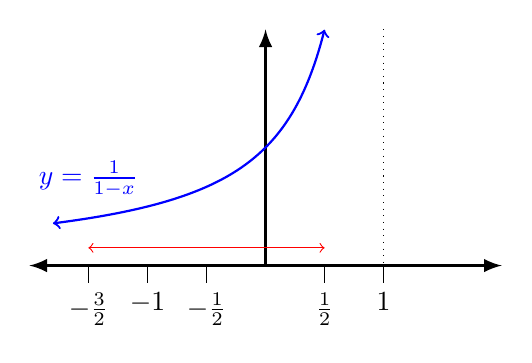
\begin{tikzpicture}[scale=1.5]
        \draw[-latex, very thick] (0, 0) -- (0, 2);
        \draw[latex-latex, very thick] (-2, 0) -- (2, 0);
        \draw[blue, thick, smooth, <->, samples = 100, domain=-1.8:0.5, variable = \x] plot(\x, {1/(1 - (\x))});
        \draw[] (1, 0) -- (1, -0.15);
        \draw[] (-1, 0) -- (-1, -0.15);
        \draw[] (-0.5, 0) -- (-0.5, -0.15);
        \draw[] (-1.5, 0) -- (-1.5, -0.15);
        \draw[] (0.5, 0) -- (0.5, -0.15);
        \node[below] at (0.5, -0.15) {$\frac{1}{2}$};
        \node[below] at (1, -0.15) {$1$};
        \node[below] at (-1, -0.15) {$-1$};
        \node[below] at (-0.5, -0.15) {$-\frac{1}{2}$};
        \node[below] at (-1.5, -0.15) {$-\frac{3}{2}$};
        \node[above, text = blue] at (-1.5, 0.5) {$y = \frac{1}{1-x}$};
        \draw[dotted] (1, 2) -- (1, -0.15);
        \draw[<->, red] (-1.5, 0.15) -- (0.5, 0.15);
    \end{tikzpicture}
    
    \caption{Plot of $y = \frac{1}{1-x}$ and region for which the Taylor series around $a = -\frac{1}{2}$ is valid (red).}
    \label{fig52}
\end{figure}
\noindent As a remark, note that although Theorem \ref{thm:8.4} only guarantees convergence up to the previous boundary, in general the Taylor series will converge up to the nearest singularity. The above theorem is a good example of \emph{analytic continuation}, where a representation of a function converges in a larger interval than the original series (notice that the above taylor series for $f$ around $a = -\frac{1}{2}$ converges up to $-\frac{3}{2}$, when the original series only converged up to $-1$). We extend the function to a larger interval.

Note that there is another way to obtain the Taylor series around $a = -\frac{1}{2}$ (in a technique reminiscent of that used in MATH 300). We can cleverly manipulate the original expression and the geometric series formula to observe that:
\begin{align*}
    f(x) = \frac{1}{1 - x} = \frac{1}{1 - x + \frac{1}{2} - \frac{1}{2}} = \frac{2}{3}\frac{1}{1 - \frac{2}{3}(x + \frac{1}{2})} = \frac{2}{3}\sum_{n=0}^\infty \left(\frac{2}{3}\right)^n (x + \frac{1}{2})^n.
\end{align*}

\begin{theorem}{Principle of Permanence of Form}{8.5}
    Suppose $\sum_n a_n x^n$ and $\sum_n b_n x^n$ each have radius of convergence larger or equal to $R$. Suppose $D \subset (-R, R)$ has a limit point in $(-R, R)$ (for example, $D = \set{\frac{R}{n}: n = 2, 3, \ldots}$ with limit point $0$). If $\sum_n a_nx^n = \sum_n b_n x^n$ in all $x \in D$, then $a_n = b_n$ for all $n \in \NN$ and $\sum_n a_nx^n$ and $\sum_n b_n x^n$ for all $x \in (-R, R)$. 
\end{theorem}
\noindent Note that this also holds for complex variables, so it can be a way of taking things we know in a real context and promoting it to a complex context. We will first prove a lemma.

\begin{nlemma}{ (Problem 2.6)}{}
    Let $E \subset X$ for a metric space $X$. Then the set $E'$ of limit points of $E$ is closed.
\end{nlemma}
\begin{nproof}
    Let $x$ be a limit point of $E'$. We wish to show that $x \in E'$. Let $\delta > 0$. Since $x$ is a limit point of $E'$, for any $r > 0$ there exists some $y \in E'$, $y \neq x$ such that $y \in N_r(x)$. Since $y \in E'$, for any $\delta - r > 0$ we have that $N_{\delta-r}(y)$ contains a point $z$ of $E$. Therefore, we have that:
    \begin{align*}
        d(x, z) \leq d(x, y) + d(y, z) < r + \delta - r = \delta
    \end{align*}
    so any neighbourhood $N_\delta(x)$ of $x$ contains some point of $E$. Hence, $x$ is a limit point of $E$ and $x \in E'$. Hence $E'$ is closed. \qed
\end{nproof}
\noindent We now move to the proof of the theorem.
\begin{nproof}
    Let $c_n = a_n - b_n$ and $f(x) = \sum_n c_nx^n$. Then, $f(x) = 0$ for all $x \in D$. Let $E = \set{x \in (-R, R): f(x) = 0}$, so $D \subset E$. We want to show that $E = (-R, R)$. Let $A = E' \cap (-R, R)$. By hypothesis, $A \neq \emptyset$ as $D$ has a limit point in $(-R, R)$. Let $B = (-R, R) \setminus A$. Then, $(-R, R) = A \cup B$ and $A \cap B = \emptyset$. By the above Lemma, the set of limit points $E'$ is closed. Hence, $A$ is closed and $B$ is open. We claim that $A$ is also open.

    To see that this is the case, we show that $E'$ is open (then $E' \cap (-R, R)$ is open as a finite intersection of open sets is open). Let $x_0 \in A$. Then, there exists $d_n$ such that $f(x) = \sum_n d_n(x - x_0)^n$ for $\abs{x - x_0} < R - \abs{x_0}$ by Theorem \ref{thm:8.4}. We will show that $d_n = 0$ for all $n$, showing that $f(x) = 0$ for all $x \in I_0 = N_{R - \abs{x_0}}(x_0)$, and therefore that $A$ is open. Suppose for the sake of contradiction that this is false. Then, there exists $k$ such that $d_k \neq 0$, i.e. $f(x) = \sum_{n=k}^\infty d_n(x - x_0)^n$ with $d_k \neq 0$. So, $f(x) = (x-x_0)^k\sum_{n=0}^\infty d_{n+k}(x - x_0)^n = g(x)$. Then, $g(x_0) = d_k \neq 0$. By the continuity of $g$, there exists $\delta > 0$ such that $g(x) \neq 0$ for $\abs{x - x_0} < \delta$. But then, $f(x) = (x - x_0)^kg(x) \neq 0$ if $0 < \abs{x - x_0} < \delta$. But then we have that there exists a neighbourhood of $x_0$ such that $f(x) \neq 0$, but then $x_0$ cannot be a limit point of $\set{x: f(x) = 0}$. So, $x_0 \notin A$, which is a contradiction. Hence $d_n = 0$ for all $n \in \NN$, and $A$ is open. 
    
    Given the claim, we have that $A \cap \overline{B} = \overline{A} \cap B = \emptyset$ and hence $A$ and $B$ are separated sets. Since $(-R, R)$ is connected and equals $A \cup B$, one of $A, B$ must be empty. It cannot be $A$ (as $E' \neq \emptyset$ by assumption) so it must be $B$. Hence $B = \emptyset$ and $A = (-R, R) = E'$. This means that any $x \in (-R, R)$ is a limit point of $E$, so there exists $\set{x_n} \subset E$ such that $x_n \rightarrow x$. Since $f$ is continuous on $(-R, R)$, we have that $f(x) = \linf f(x_n) = 0$. So, $x \in E$ and $E = (-R, R)$. \qed
\end{nproof}
\noindent Having proven some more properties of power series, we now move to formal definitions of the exponential/logarithmic/trigonometric functions and a from-first-principles proof of their properties. 

\subsection{: The Exponential Function}
Recall Definition \ref{def:3.30}, where we defined $e = \sum_{n=0}^\infty \frac{1}{n!}$. We also showed in Theorem \ref{thm:3.31} that $e = \linf\left(1 + \frac{1}{n}\right)^n$. We also know that $2 < e < 3$, and  by Theorem \ref{thm:3.32} that $e$ is irrational. We now define a power series based on $e$. 

\begin{ndef}{: The Exponential Function}{}
    For $z \in \CC$, we define:
    \begin{align*}
        E(z) = \sum_{n=0}^\infty \frac{z^n}{n!}
    \end{align*}
\end{ndef}
\noindent In particular, we note that $E(1) = e$. Also note that (from Example \ref{exam:3.40}) that the above power series has radius of convergence $R = \infty$. We will show with the next sequence of theorems that $E(z)$ coincides with the exponential function $\exp(z) = e^z$ that we are familiar with.

\begin{ntheorem}{: Addition Formula}{}
    For $z, w \in \CC$, we have that $E(z + w) = E(z)E(w)$.
\end{ntheorem}
\begin{nproof}
    From the defintion, we have that:
    \begin{align*}
        E(z)E(w) &= \sum_{n=0}^\infty \frac{z^n}{n!}\sum_{m=0}^\infty\frac{w^m}{m!}
        \\ &= \sum_{n=0}^\infty \sum_{k=0}^n \frac{z^k}{k!}\frac{w^{n-k}}{(n-k)!}
        \\ &= \sum_{n=0}^\infty \frac{1}{n!}\sum_{k=0}^n\binom{n}{k}z^kw^{n-k}
        \\ &= \sum_{n=0}^\infty \frac{1}{n!}(z + w)^n
        \\ &= E(z + w)
    \end{align*}
    where in the second equality we use Theorem \ref{thm:3.50} for the multiplication of series. \qed
\end{nproof}
\noindent We can now use this addition formula to show how $E(p)$ coincides with $\exp(p)$:

\begin{ntheorem}{}{}
    For $p \in \QQ, E(p) = e^p$. 
\end{ntheorem}
\begin{nproof}
    Setting $z = w = 1$ in the addition formula above, we note that:
    \begin{align*}
        E(2) = E(1 + 1) = E(1)^2 = e^2, \quad E(3) = E(2 + 1) = E(2)E(1) = e^2e^1 = e^3
    \end{align*}
    so by induction, it follows that for $N \in \NN$:
    \begin{align*}
        E(N) = e^N
    \end{align*}
    Furthermore, we observe that:
    \begin{align*}
        E(z)E(-z) = E(z - z) = E(0) = 1
    \end{align*}
    so it follows that $E(z) = \frac{1}{E(z)}$. Hence, $E(-N) = \frac{1}{e^N} = e^{-N}$ for $N \in \NN$. Finally, let $p = \frac{m}{n}$ with $m, n \in \NN$. Then, we have that:
    \begin{align*}
        e^m = E(m) = E(np) = E(p + \ldots + p) = E(p)^n
    \end{align*}
    so therefore:
    \begin{align*}
        E(\frac{m}{n}) = E(p) = e^{\frac{m}{n}}
    \end{align*}
    Additionally, we have that:
    \begin{align*}
        1 = E(p - p) = E(p)E(-p) = e^pE(-p) \implies E(-p) = \frac{1}{e^p}.
    \end{align*}
    We have hence successfully shown that $E(p) = e^p$ for $p \in \QQ$. \qed
\end{nproof}
\noindent Next, we will extend the theorem for real exponents and study properties. We will have to come up with a different definition for an exponential of irrational powers; note that so far, our definition for exponentials $a^x$ only could accomodate rational $x$. 

\begin{ndef}{: Real Exponentials}{}
    For $x \in \RR$, let:
    \begin{align*}
        e^x = E(x) = \sum_{n=0}^\infty \frac{x^n}{n!}
    \end{align*}
\end{ndef}
\noindent The above defintion defines $x \mapsto e^x$ as an analytic function on $\RR$, which is therefore infinitely differentiable on $\RR$. Futhermore, the derivatives have a certain property.
\begin{ntheorem}{}{}
    $\od{}{x}e^x = e^x$.
\end{ntheorem}
\begin{nproof}
    By the defintion of $e^x$ we have that:
    \begin{align*}
        \dod{}{x}e^x = \sum_{n=0}^\infty \dod{}{x}\left(\frac{x^n}{n!}\right) = \sum_{n=0}^\infty \left(\frac{nx^{n-1}}{(n-1)!}\right) = \sum_{n=1}^\infty \frac{x^{n-1}}{(n-1)!} = \sum_{n=0}^\infty \frac{x^n}{n!} = e^x
    \end{align*}
\end{nproof}

\begin{ntheorem}{}{}
    $e^x > 0$ for all $x \in \RR$.
\end{ntheorem}
\begin{nproof}
    Since $e^{x+y} = e^xe^y$ by the addition formula, we have for any $x \in \RR$ that $e^{x}e^{-x} = 1$. Since $e^x > 0$ if $x \geq 0$ by definition, it follows that $e^{-x} > 0$ as well if $e^{x}e^{-x} = 1 > 0$ is to be satisfied. \qed
\end{nproof}

\begin{ntheorem}{}{}
    $e^x$ is strictly increasing and strictly convex.
\end{ntheorem}
\begin{nproof}
    Since $\od{}{x} e^x = e^x > 0$ and $\od[2]{}{x} e^x = e^x > 0$ by the two previous theorems, we conclude that $e^x$ is strictly increasing and convex by Theorems \ref{thm:5.11} (and its extension).
\end{nproof}

\begin{ntheorem}{: Superpolynomial Asymptotic Growth}{}
    $\lim_{x \rightarrow \infty} \frac{e^x}{x^n} = \infty$.
\end{ntheorem}
\begin{nproof}
    For $n \geq 0$, the defintion shows that:
    \begin{align*}
        e^x > \frac{x^{n+1}}{(n+1)!}
    \end{align*}
    if $x > 0$, as on the RHS we drop all but the $k = n+1$ term in the series (and all of the terms are positive for $x > 0$). Rearranging, we have that:
    \begin{align*}
        \frac{e^x}{x^n} > \frac{x}{(n+1)!}
    \end{align*}
    and the claim follows by taking $x \rightarrow \infty$. \qed
\end{nproof}
\noindent The above theorem shows that $e^x$ grows faster than any power of $x$. We also obtain the Corollary:
\begin{ncorollary}{}{}
    $\lim_{x \rightarrow \infty} e^x = \infty$, $\lim_{x \rightarrow \infty} e^{-x} = 0$. 
\end{ncorollary}
\begin{nproof}
    The first claim follows by setting $n = 0$ in the previous Theorem, and the second by using that $e^{-x} = \frac{1}{e^x}$. \qed
\end{nproof}
\noindent Since $e^x$ is strictly increasing, we may now define an inverse of $e^x$ at each $y > 0$. 

\subsection{The Logarithm}

\subsection{Sine and Cosine}

\subsection{The Fundamental Theorem of Algebra}

\subsection{Fourier Series}